\begin{myact}{2 Classement}
	Activité 3 page 13
\end{myact}

\begin{myactrep}{2 Classement}
	\begin{enumerate}
		\item Le colis le plus lourd est celui qui a une masse de \num{15.3} kg et \num{13.999} kg pour le plus léger.
		\item On a donc :
		
		\num{13.999} < \num{14.15} < \num{14.509} < \num{14.575} < \num{14.59} <  \num{14.805} < \num{15.29} < \num{15.3}
	\end{enumerate}
\end{myactrep}

\begin{mydefs}
	\begin{itemize}
		\item \kw{Comparer} des nombres, c'est dire si un est plus petit ou plus grand que l'autre ou s'ils sont égaux.
		
		\item Ranger des nombres du plus petit au plus grand, c'est les classer par \kw{ordre croissant}.
		
		\item Ranger des nombres du plus grand au plus petit, c'est les classer par \kw{ordre décroissant}.
		
		\item \kw{Encadrer} un nombre, c'est trouver un nombre plus petit \textbf{et} un nombre plus grand que ce nombre.
		
		\item \kw{Intercaler} un nombre entre deux autres, c'est un nombre compris entre ces deux nombres.
	\end{itemize}
\end{mydefs}

\begin{myexs}
	\begin{itemize}
		\item 42 < 128, \pause se lit <<42 est inférieur à (ou plus petit que) 128>>;\pause
		\item 1337 < 1024,\pause se lit <<\num{1337} est supérieur à (ou plus grand que) \num{1024}>>;\pause
		\item 2 < \num{3.2} < \num{6.4} < \num{25.6} : ces nombres sont rangés dans l'ordre \pause croissant;\pause
		\item 123 > \num{45.6} > \num{7.89} > \num{5} : ces nombres sont rangés dans l'ordre \pause décroissant;\pause
		\item Encadrement de 21 à l'unité près : \pause 20 < 21 < 22 ;\pause
		\item Encadrement de \num{21.987} au centième près : \pause \num{21.977} < \num{21.987} < \num{21.997} ;\pause
	\end{itemize}
\end{myexs}

\begin{myexos}
	\begin{itemize}
		\item \Exo{16}{18} : Intercaler des nombres;
		\item Exercices 17 et 18 page 18 : Comparer des nombres;
		\item \Exo{19}{18} : Ordre croissant
		\item \Exo{20}{18} : Ordre décroissant
		\item Exercices 23 et 24 page 18 : Encadrer des nombres;
		\item \Exo{25}{19} : Comparer des nombres;
		\item \Exo{26}{19} : Ordre croissant;
		\item \Exo{27}{19} : Ordre décroissant.
	\end{itemize}
\end{myexos}


\begin{myprop}
	Un point placé sur une demi-droite graduée est repéré par un nombre, son \kw{abscisse}.
\end{myprop}

\begin{myex}
	\begin{center}
		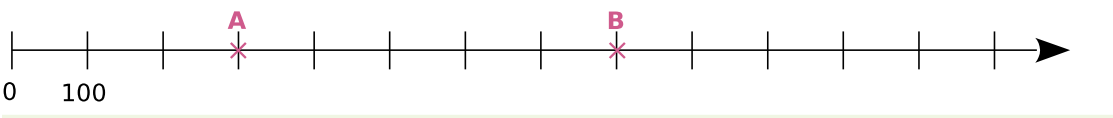
\includegraphics[scale=0.5]{img/axe}
	\end{center}

	\begin{itemize}
		\item L'abscisse du point A est :
		\item L'abscisse du point B est :
		\item L'abscisse du point C est : 500;
		\item L'abscisse du point D est \num{1100}.
	\end{itemize}
\end{myex}